This chapter will describe the requirements of the application as a whole. The structure of this chapter roughly follows the SRS Template as proposed by Wiegers in Chapter 11 and Appendix D of \cite{wiegers2013software}.

\section{Vision and Scope}

    \subsection{Background}

        Melanoma is a type malignant skin tumour that develops from benign melanocytic nevi. Although less frequent than other skin cancer types, it causes more deaths \cite{cancer_gov_skin}, and it’s incidence is increasing dramatically, especially in the young white population \cite{S_ez_2013}. Early diagnosis and treatment is vital.

Several non-invasive techniques exist which dermatologist can employ to visually make a diagnosis. The most common are pattern analysis, the ABCD rule, the 7-point checklist and the Menzies method, among others \cite{marghoob2004atlas}. These methods generally use a combination of defined visual clues and indicators to assess the risk of a skin lesion. CAD ( Computer Aided Diagnosis ) systems exists that can assist a dermatologist, and even provide automatic diagnosis with an accuracy comparable to that of doctors trained in dermoscopic techniques \cite{Filho2015}.

    \subsection{Business Case}

        A smart phone based assistant would provide a valuable service by making it easy, painless, inexpensive, and fast to get a preliminary risk assessment of a skin lesion. It is too easy to postpone making an appointment with a dermatologist to have a suspect lesion examined. Visiting an dermatologist is not on most people’s list of fun things to do in the spare time, it requires time and effort. By the time a lesion is visually compelling enough, it might be too late.

A smart phone based application that could make a preliminary diagnosis in near real time would be a great time save and offer compelling enough information to actually make the appointment with a dermatologist.

    \subsection{Scope and Limitations}
    \subsubsection{Major Features}
        \noindent
        \begin{itemize}[leftmargin=*]
            \item[]  \textbf{FE-1} : The smart phone app allows the user to capture and analyse an image of a skin lesion and provide a risk assessment to the user of the lesion being a malignant melanoma.

            \item[] \textbf{FE-2} : The app allows the user to create, view, edit or delete metadata that is associated with an image and corresponding risk assessment.

            \item[] \textbf{FE-3} : The app allows the user to save or archive the image and corresponding assessment for future comparison and review.

            \item[] \textbf{FE-4} : The user can browse archived images, assessments, and associated metadata.

            \item[] \textbf{FE-5} : The user can send a set of images with associated assessment and metadata via email.

            \item[] \textbf{FE-6} : The app will run on all popular smart phone devices and systems.

            \item[] \textbf{FE-7} : The analysis algorithms employed by the app should be easily updatable and extendable.
        \end{itemize}

        \begin{figure}[H]
            \centering
            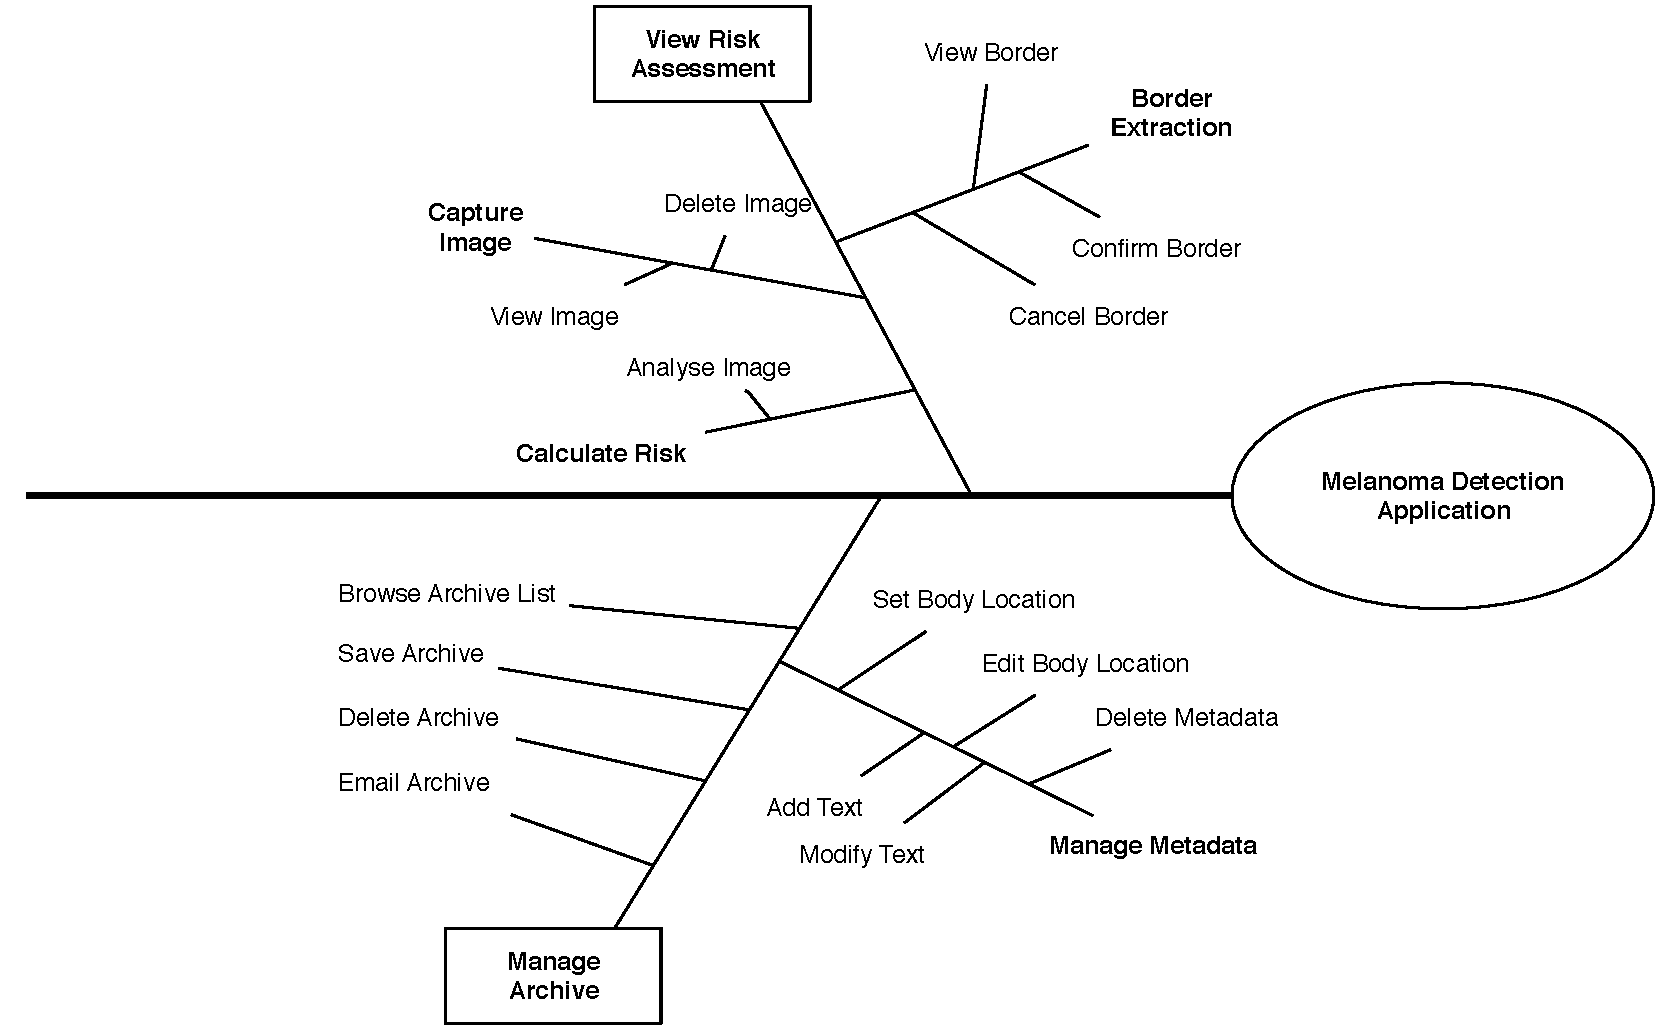
\includegraphics[width=\textwidth]{assets/requirements/PartialFeatureTree.pdf}
            \caption{Partial Feature Tree for the Melanoma Detection App}
            \label{fig:partial_feature_tree}
        \end{figure}


    \subsubsection{Stakeholder Profile}




    \subsection{Use Cases}

        \begin{figure}[H]
            \centering
            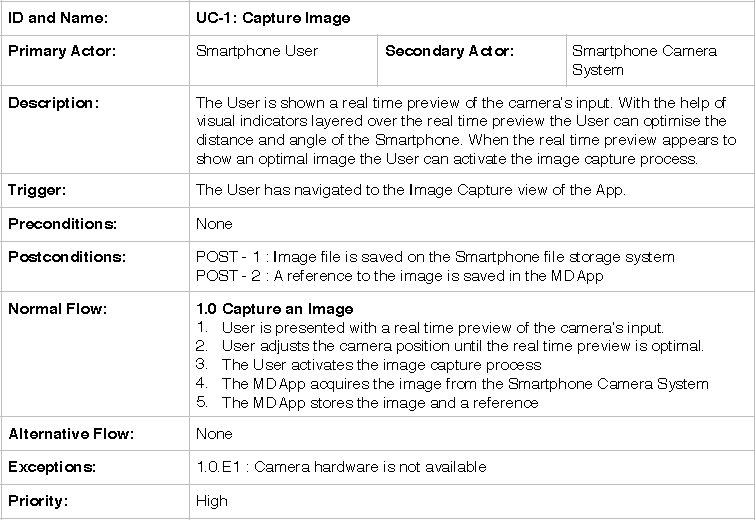
\includegraphics[width=\textwidth]{assets/requirements/uc/usecase_01.pdf}
            \caption{UC-1}
            \label{fig:uc-1}
        \end{figure}
        \begin{figure}[H]
            \centering
            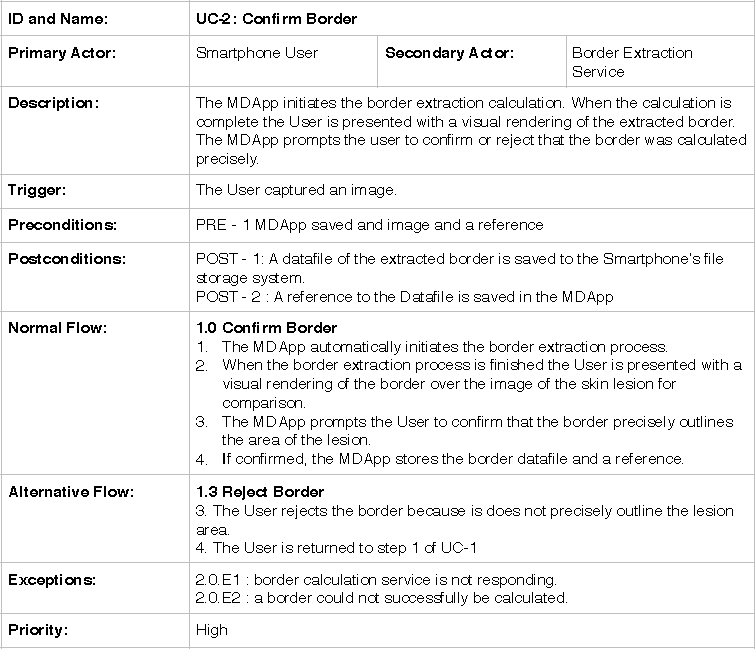
\includegraphics[width=\textwidth]{assets/requirements/uc/usecase_02.pdf}
            \caption{UC-2}
            \label{fig:uc-2}
        \end{figure}
        \begin{figure}[H]
            \centering
            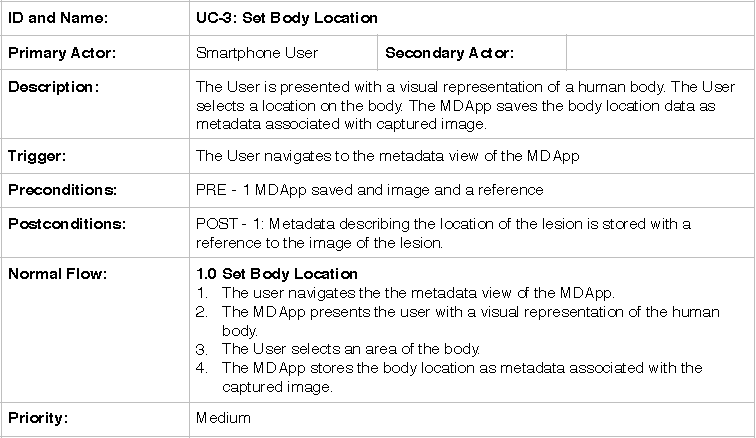
\includegraphics[width=\textwidth]{assets/requirements/uc/usecase_03.pdf}
            \caption{UC-3}
            \label{fig:uc-3}
        \end{figure}
        \begin{figure}[H]
            \centering
            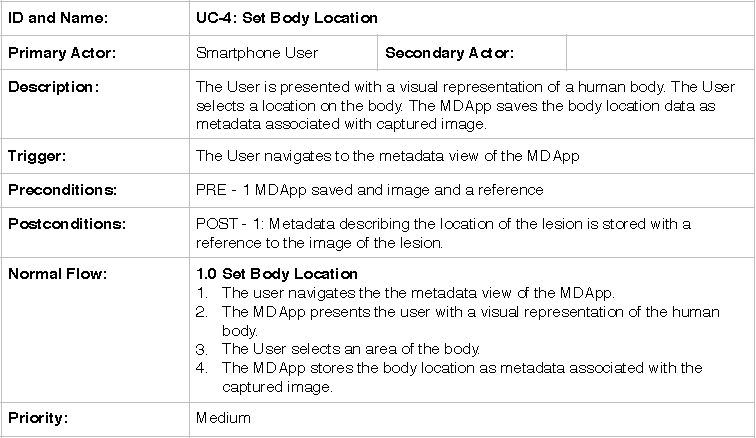
\includegraphics[width=\textwidth]{assets/requirements/uc/usecase_04.pdf}
            \caption{UC-4}
            \label{fig:uc-4}
        \end{figure}
        \begin{figure}[H]
            \centering
            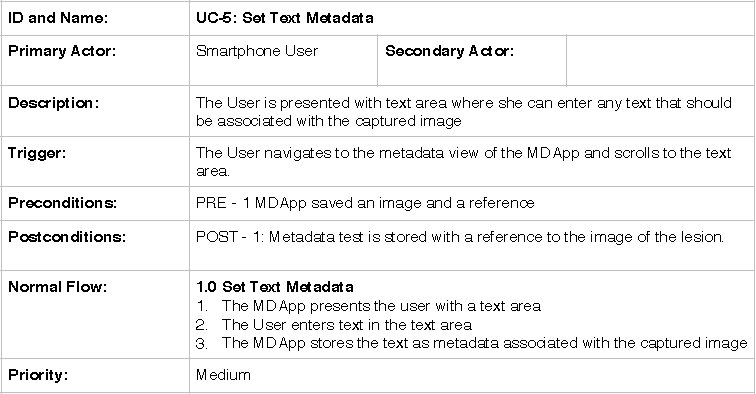
\includegraphics[width=\textwidth]{assets/requirements/uc/usecase_05.pdf}
            \caption{UC-5}
            \label{fig:uc-5}
        \end{figure}
        \begin{figure}[H]
            \centering
            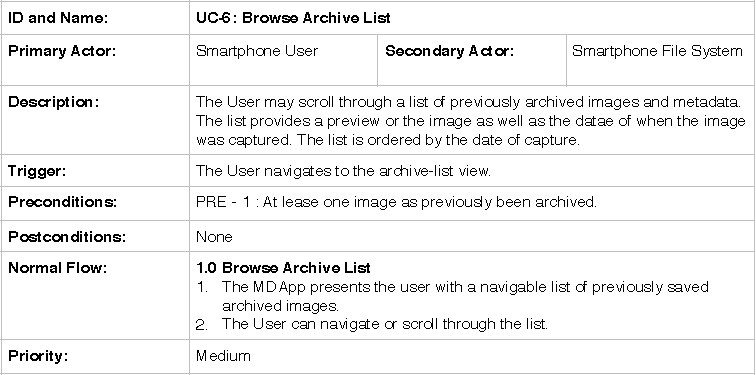
\includegraphics[width=\textwidth]{assets/requirements/uc/usecase_06.pdf}
            \caption{UC-6}
            \label{fig:uc-6}
        \end{figure}
        \begin{figure}[H]
            \centering
            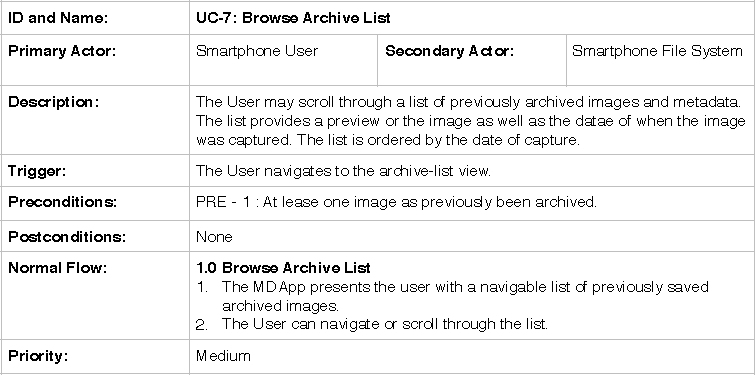
\includegraphics[width=\textwidth]{assets/requirements/uc/usecase_07.pdf}
            \caption{UC-7}
            \label{fig:uc-7}
        \end{figure}
        \begin{figure}[H]
            \centering
            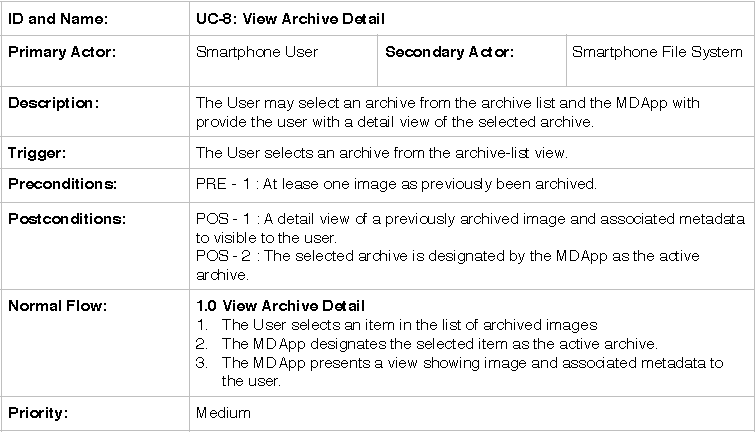
\includegraphics[width=\textwidth]{assets/requirements/uc/usecase_08.pdf}
            \caption{UC-8}
            \label{fig:uc-8}
        \end{figure}

\section{Software Requirements Specification}

    \subsection{Introduction}

        \subsubsection{Purpose}

            The Software Requirements Specification will describe the functional and nonfunctional requirements of the Melanoma Detection App. It is meant to be a guideline for developers who will be implementing the mobile application.

    \subsection{Overall Description}

        \subsubsection{Product Perspective}

            The Melanoma Detect App will provide the user with a risk assessment of a skin lesion. The App will guide the user through the process of capturing an image and confirming the correct recognition of the boundary of the lesion. Once confirmed the App will analyse the visual features of the lesion based on dermatological rules and provide the user with an initial risk assessment.

    The App should help motivate the user to make an appointment with a dermatologist when a significant risk has been detected. It is not meant to replace the need to visit a dermatologist though.


            \begin{figure}[H]
                \centering
                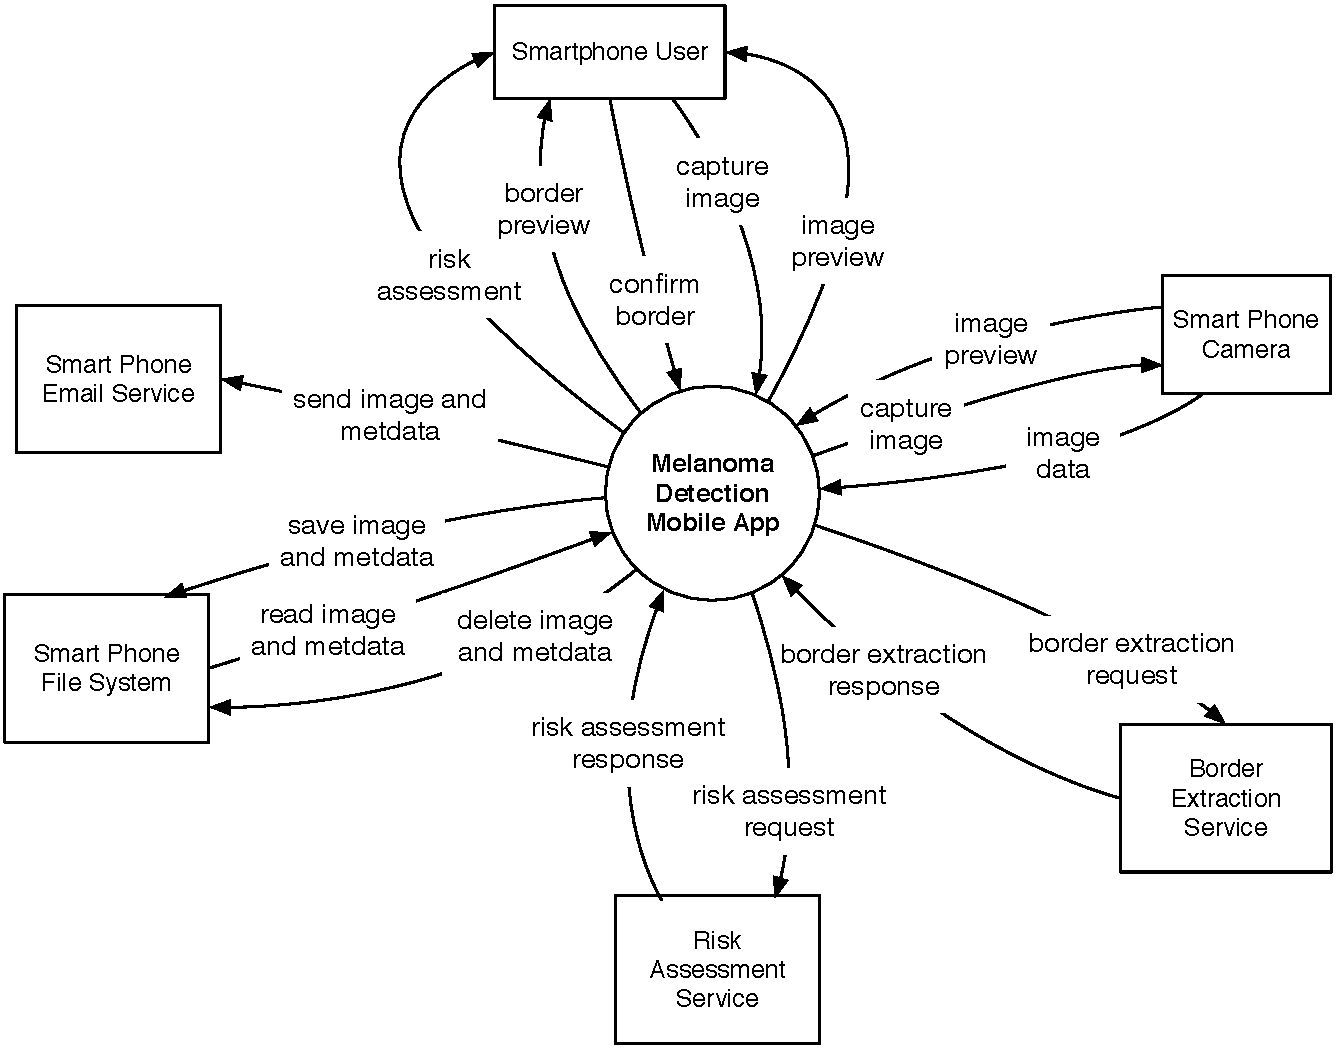
\includegraphics[width=\textwidth]{assets/requirements/ContextDiagram.pdf}
                \caption{Context Diagram of the Melanoma Detection App}
                \label{fig:partial_feature_tree}
            \end{figure}


        \subsubsection{User Classes and Characteristics}

            The Melanoma Detection App only has one class of user, the Smartphone User. The Smartphone User has one or several skin lesions that she or he is worried about.
The Smartphone User is not expected to have any technical or dermatological expertise.

        \subsubsection{Operating Environment}

                    \noindent
                    \begin{itemize}[leftmargin=*]
                        \item[]  \textbf{OE-1} : The Mobile App shall operate on the following platforms: Android OS (v.5.2.2) and iOS (v. 9.3)

                    \end{itemize}


        \subsubsection{Design and Implementation Constraints}

                    \noindent
                    \begin{itemize}[leftmargin=*]
                        \item[]  \textbf{CO-1} : The Border Extraction and Risk Assessment Services shall be implemented on a server in oder to leverage the effort already made with python and python based libraries for image processing and scientific calculations. Wifi access is therefore a requirement for the app to run.
                        \item[]  \textbf{CO-2} : The method for archiving images and risk assessment data will use whatever standard is the most accepted for the relevant platform. i.e. iCloud on iOS.


                    \end{itemize}


        \subsubsection{Assumptions and Dependencies}

                    \noindent
                    \begin{itemize}[leftmargin=*]
                        \item[]  \textbf{AS-1} : It is assumed that the user of the software is also the user of the mobile phone. The software might need to request permission from the user to access the camera or network.

                    \end{itemize}


    \subsection{System Features}

        \subsubsection{Capture an Image of a Skin Lesion}

                \begin{figure}[H]
                    \centering
                    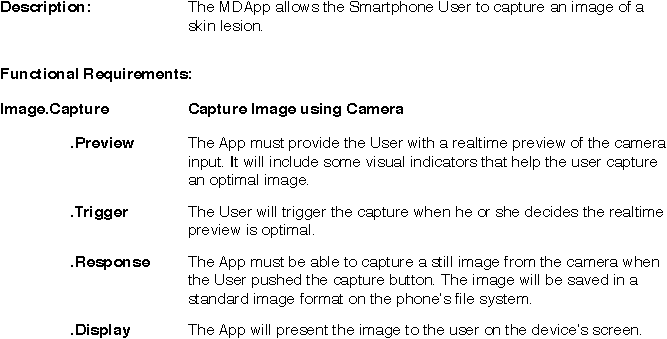
\includegraphics[width=\textwidth]{assets/requirements/req/ImageCapture.pdf}
                    \label{fig:image.capture}
                \end{figure}

        \subsubsection{Extract the Border of a Skin Lesion in an Image}

                \begin{figure}[H]
                    \centering
                    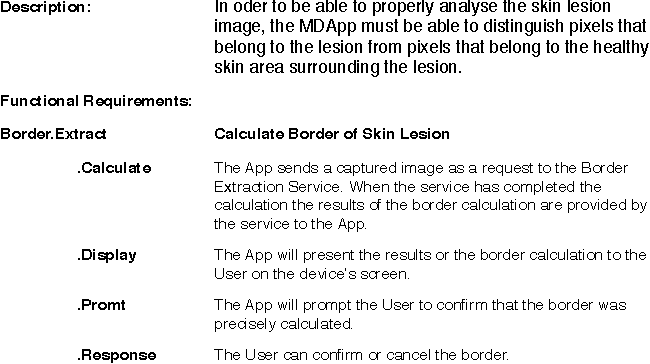
\includegraphics[width=\textwidth]{assets/requirements/req/BorderExtract.pdf}
                    \label{fig:image.capture}
                \end{figure}

        \subsubsection{Calculate the Risk Assessment of a Skin Lesion Image}
        \subsubsection{Create, Modify, and Delete Skin Lesion Image Metadata}
        \subsubsection{Save, View, Edit, and Delete Skin Lesion Archive}


    \subsection{Data Requirements}
        \subsubsection{Logical Data Model}
        \subsubsection{Data Dictionary}
        \subsubsection{Reports}






